\documentclass[11pt]{article}

\usepackage[utf8]{inputenc} % Required for inputting international characters
\usepackage[T1]{fontenc} % Output font encoding for international characters
\usepackage{graphicx}
\usepackage{float}
\usepackage{hyperref}
\usepackage{amsmath}
\usepackage{cite}
\usepackage{pdfpages}
\usepackage[german]{varioref}
\usepackage{mathpazo} % Palatino font
\usepackage[german]{babel}
\parindent0pt
\pdfinclusioncopyfonts=1

\begin{document}

\begin{titlepage} % Suppresses displaying the page number on the title page and the subsequent page counts as page 1
	\newcommand{\HRule}{\rule{\linewidth}{0.5mm}} % Defines a new command for horizontal lines, change thickness here
	
	\center % Centre everything on the page
	\vspace*{0.75cm}
%\includegraphics[width=0.8\textwidth]{../tex/fu_logo}\\[1cm] 

%\textsc{\LARGE  Freie Universität Berlin}\\[1.5cm] % Main heading such as the name of your university/college
	
	\textsc{\Large Neurobiologie für BioinformatikerInnen: Praktikum B}\\[0.65cm] % Major heading such as course name
	
	\textsc{\large Protokoll zum 2. Praktikumstag am 14.01.2019}\\[0.65cm] % Minor heading such as course title

	\HRule\\[0.5cm]
	
	{\huge\bfseries Erregungsleitung im Bauchmark des Regenwurms}\\[0.3cm] % Title of your document
	
	\HRule\\[0.75cm]
	\textsc{\Large\bfseries Gruppe IV}
	\\[0.8cm]
	
\vfill

	\begin{minipage}{0.45\textwidth}
		\begin{flushleft}
			\large
			\textit{Gruppenmitglieder}\\
			\textsc{Alia Rothkegel}\\
			\textsc{Mara Steiger}
			 % Your name
		\end{flushleft}
	\end{minipage}
	~
	\begin{minipage}{0.45\textwidth}
		\begin{flushright}
			\large \vspace{16pt}
			alia.rothkegel@fu-berlin.de\\
			mara.steiger@fu-berlin.de 
		\end{flushright}
	\end{minipage}
	
\vfill

	\begin{minipage}{0.45\textwidth}
		\begin{flushleft}
			\large
			\textit{Lehrveranstalter}\\
			Prof. Dr. P.R. \textsc{Hiesinger}\\ 
			Dr. D. \textsc{Malun}\\ 
			Prof. Dr. M. \textsc{Wernet}
		\end{flushleft}
	\end{minipage}
	~
		\begin{minipage}{0.45\textwidth}
		\begin{flushright}
			
		\end{flushright}
	\end{minipage}
\vfill
	\begin{minipage}{0.7\textwidth}
		\begin{flushleft}
			\large
			\textit{TutorInnen}\\
			\textsc{Lisa Peters}\\
			\textsc{Johannes Brüner Hammacher}\\
			\textsc{Claudia Haushalter}
		\end{flushleft}
	\end{minipage}
	~
		\begin{minipage}{0.2\textwidth}
		\begin{flushright}
			
		\end{flushright}
	\end{minipage}

	% If you don't want a supervisor, uncomment the two lines below and comment the code above
	%{\large\textit{Author}}\\
	%John \textsc{Smith} % Your name
	\vfill\vfill\vfill % Position the date 3/4 down the remaining page

	
	\vfill % Push the date up 1/4 of the remaining page
	
\end{titlepage}

%----------------------------------------------------------------------------------------
\section{Einleitung}
Ziel der heutigen Experimente ist es, die Erregungsleitung und Funktionsweise der dorsalen Riesenaxone des Regenwurmes zu untersuchen. 

\subsection{Erregungsleitung in Nervenzellen}
Die Fortleitung von Informationen wird von Zellen des Nervensystem übernommen und basiert auf Spannungsunterschieden zwischen dessen Zellinnerem und dem extrazellulären Raum. \\
Aufgrund der Semipermeabilität der Membran von Neuronen liegt ein sogenanntes Ruhepotential von ca. -70mV vor. Die Membran ist für größere Ionen wie Natrium ($Na^{+}$) nicht permeabel, aber Kalium ($K^{+}$) kann frei diffundieren. Daher entspricht das Ruhemembranpotential in etwa dem Gleichgewichtspotential von Kalium. Durch die geringere Konzentration von Kalium-Ionen außen ergibt sich ein negatives Membranpotential, d.h. die Nervenzelle ist gegenüber der Außenseite negativ geladen. Außerdem trägt eine Natrium-Kalium-Pumpe ($Na^{+}$-$K^+$-ATPase) zum Erhalt des Membranpotentials bei.  \\
Eine Nervenzelle wird durch die Bindung eines Neurotransmitters an einen ligandengesteuerten Ionenkanal in der Plasmamembran aktiviert. Dieser Kanal öffnet sich durch die Bindung, woraufhin $Na^{+}$ entlang des Konzentrationsgradienten in die Zelle einströmt und eine Depolarisation bewirkt. Spannungsabhängige $Na^{+}$-Kanäle entlang des Axons einer Nervenzelle, die durch die Depolarisation in benachbarten Regionen der Zelle kurz geöffnet werden, sorgen für die Ausbreitung des Aktionspotentials in Form einer Depolarisationswelle durch das Neuron. Kurz nach der Depolarisation durch den Natrium-Einstrom öffnen sich auch spannungsgesteuerte $K^+$-Kanäle entlang des Axons, die wiederum eine Repolarisation durch den Ausstrom von Kalium bewirken. Da diese Kalium-Kanäle etwas langsamer schließen, kommt es zu einer Hyperpolarisation der Zelle. Anschließend wird das Ruhepotential durch Leckströme von Ionen und die Aktivität der Natrium-Kalium-Pumpe wiederhergestellt.  \cite{lehninger}
\begin{figure}[H]
\makebox[\textwidth][c]{\includegraphics[width=0.85\textwidth]{aktionspotential}}
\caption{Die Abbildung zeigt den zeitlichen Verlauf eines Aktionspotentials einer Nervenzelle. Zu sehen ist die Depolarisation von -70mV auf ca. +20mV, danach die Repolarisation übergehend zur Hyperpolarisation zu ca. 100mV und die Wiederherstellung des Ruhepotentials.  }
\label{ap}
\end{figure}

Die passiven elektrischen Eigenschaften der Nervenzelle beeinflussen hierbei die Geschwindigkeit, mit der sich ein Aktionspotential ausbreitet. Dies ist zum einen der Membranwiderstand $R_m$, zum anderen die Membrankapazität $C_m$ und außerdem der intrazelluläre Längswiderstand $R_i$. Außerdem wirkt sich der Durchmesser eines Neurons auf die Fortleitungsgeschwindigkeit aus.  \cite{haustiere} 

\subsection{Refraktärphase}\label{refraktär}
Nachdem die Natrium-Kanäle während der Depolarisation kurz geöffnet waren, sind sie für eine bestimmte Zeit inaktiviert. Diese Phase nennt man Refraktärphase. Währenddessen können diese Natrium-Kanäle nicht aktiviert werden und ein weiteres Aktionspotential auslösen. Dadurch wird erreicht, dass sich die Depolarisationswelle, d.h. das Aktionspotential, nur in eine Richtung entlang des Axons ausbreitet.  \cite{zellbiologie} \\
Man unterscheidet zwischen der absoluten und relativen Refraktärphase. Während der absoluten Refraktärphase ist eine Erregung überhaupt nicht möglich, auch nicht durch eine starke Depolarisation. \\
Die relative Refraktärphase beginnt direkt nach der absoluten Refraktärphase. Hier ist eine erneute Erregung zwar möglich, aber das Schwellenpotential ist deutlich höher. Das heißt, um erneut ein Aktionspotential auszulösen ist ein stärkerer Reiz nötig. Außerdem ist während dieser Zeit die Amplitude des resultierenden Aktionspotentials verringert. \cite{physiologie}

\subsection{Riesenaxone}
Die Entwicklung von Axonen mit deutlich größerem Durchmesser ist durch den evolutiven Vorteil entstanden, dass diese Aktionspotentiale schneller fortleiten können. Besonders für Bewegungsabläufe, die bei Fluchtreaktionen von Bedeutung sind, ist diese Eigenschaft entscheidend. \\
Bei der Vergrößerung des Durchmessers von Nervenfasern kommt es zu einem geringeren cytoplasmatischen Längswiderstand $R_i$, der wiederum für einen Anstieg der Längskonstante $\delta$ verantwortlich ist. Der Längswiderstand $R_i$ lässt sich wie folgt berechnen:
\begin{equation}
\label{eq1}
R_i = \dfrac{R_m}{\pi d^2}
\end{equation}
Daraus folgt, dass bei gleichem Membranwiderstand $R_m$ die Längskonstante $R_i$ für einen steigenden Durchmesser sinkt. Ursache dafür ist, dass durch den größeren Durchmesser der Widerstand, der sich in der Zelle dem Stromfluss (einströmenden Ionen) entgegenstellt, geringer ist. \\
Die Längskonstante $\lambda$ ist die Strecke, in der die maximale Amplitude der Spannungsänderung durch die Depolarisation auf den Anteil $\frac{1}{e} \approx 37\%$ abgefallen ist.  \cite{physiologie} Sie berechnet sich folgendermaßen:
\begin{equation}
\label{eq2}
\lambda = \dfrac{d/2 \cdot R_m}{2 R_i} = \dfrac{d \cdot R_m}{4 R_i}
\end{equation}
Demnach kann das Aktionspotential eine größere Distanz überbrücken, bis es seine Amplitude verliert, wenn der Durchmesser des Axons größer ist. \\
Diese Eigenschaften führten zur positiven Selektion von Riesenfasern, die man heute noch bei Arten der Bilateria finden kann. 

\subsection{Myelinisierung}
Um den Längswiderstand $L_i$ zu erhöhen, kann auch der Membranwiderstand $R_m$ bei gleichbleibendem Durchmesser $d$ vergrößert werden (\vref*{eq1}). \\
Dies wird bei der Myelinisierung über eine saltatorische Erregungsleitung erreicht, bei der im Gegensatz zu nicht-myelinisierten Axonen die aktiven und passiven Leitungsmechanismen zeitlich und räumlich voneinander getrennt sind. \\
Gliazellen umhüllen Axone und bilden die Myelinscheide, indem sie sich um die Nervenfaser wickeln. Dadurch wird das Axon isoliert und es liegt ein größerer Membranwiderstand vor, sodass der Längswiderstand verringert wird und schließlich eine Erhöhung der Längskonstante bewirkt wird (\vref*{eq2}). \\
Die myelinisierten Nervenfasern weisen sogenannte Ranvier-Schnürringe auf, an denen die aktiven Leitungsprozesse (langsamere Erregungsleitung) ablaufen , während die passiven in den isolierten Abschnitten (schnelle Erregungsleitung) erfolgen. An diesen Schnürringen liegt das Axon unmyelinisiert vor, diese kurzen Abschnitte dienen zur Regeneration der Amplitude des Aktionspotentials. \cite{physiologie}

\begin{figure}[H]
\makebox[\textwidth][c]{\includegraphics[width=0.85\textwidth]{myelin}}
\caption{Dies ist eine schematische Darstellung einer myelinisierten Nervenfaser. Gezeigt ist, wie ein Aktionspotential von einem zum nächsten Schnürring \glqq springt\grqq{}. }
\label{myelin}
\end{figure}


\subsection{Anatomie des Lumbricus terrestris}\label{anatomie} 
Der gemeine Regenwurm (auch: Tauwurm) \textit{Lumbricus terrestris} besitzt einen länglichen, bräunlich rot gefärbten Körper, der in mehrere Segmente unterteilt ist. Zur Fortbewegung befinden sich an jedem dieser Segmente zwei Borstenpaare an der Unterseite. Das vordere Ende weist eine dunklere, eher braune Färbung auf und läuft spitz zu, während das hintere Ende eher heller gefärbt ist. Der Körper des Regenwurms besteht aus einer flüssigkeitsgefüllten, sekundären Leibeshöhle oder \textit{Coelom}, die von einem formgebenden Hautmuskelschlauch umgeben ist. In der Leibeshöhle befinden sich auch die Organe des Regenwurms, sprich der Darm, die Gonaden, die Nephriden, das Ringgefäß mit Rücken- sowie Bauchgefäß und das für diesen Versuch relevante Bauchmark (siehe Abbildung \ref{bauchmark}). \cite{koerperbau}
\begin{figure}[H]
\makebox[\textwidth][c]{\includegraphics[width=0.7\textwidth]{bauchmark-laengs}\hspace*{4mm}\includegraphics[width=0.35\textwidth]{bauchmark-quer}}%\makebox[\textwidth][c]{}
\caption{Die Skizze zeigt die Anatomie des Regenwurms, links im Längs- und rechts im Querschnitt. Das Bauchmark ist gelb hervorgehoben.}
\label{bauchmark}
\end{figure}
Im Bauchmark befinden sich die Riesenfasern des Regenwurms: die mediane Riesenfaser (im Folgenden als MRF bezeichnet) und die lateralen Riesenfasern (im Folgenden als LRF bezeichnet). Zusätzlich zu dem vergrößerten Durchmesser der in ihnen liegenden Neuronen sind die Riesenfasern myelinisiert. Die beiden LRF mit je einem Durchmesser von ca. $50 \mu m$, der zu anterior abnimmt, sind über Querbrücken verbunden und fungieren so wie eine einzelne Nervenfaser. Die MRF hat einen Durchmesser von ca. $75 \mu m$, der Richtung posterior abnimmt. Sie erfüllen unterschiedliche Funktionen und sprechen so unterschiedliche sensorische und motorische Neuronen an. Die MRF sorgt bei Reizen am anterioren Pol für das Abflachen des posterioren Körperendes und somit für ein Zurückziehen des anterioren Körperendes. Die LRF sorgen bei einem Reiz am posterioren Ende dafür, dass sich der Wurm am anterioren Ende "{}festhält"{} und das posteriore Ende wegzieht.\cite{skript}

\subsection{Differentielle Ableitung}\label{differentiell}
Eine differentielle Ableitung ist eine Methode zur Ableitung elektrischer Muskelpotentiale, bei der eine lokale Spannungsdifferenz zwischen zwei Elektroden gemessen wird. Dies dient dem Herausfiltern von Störsignalen der elektromagnetischen Wechselfelder der Umwelt. Es wird angenommen, dass sich diese Störsignale ca. mit Lichtgeschwindigkeit ausbreiten und somit beide Elektroden zur gleichen Zeit erreichen. Berechnet man nun die Differenz der von den Elektroden jeweils gemessenen Spannungen, so ergibt sich folgende Gleichung:
\begin{center}
$U_{ges}= (U_1+S_1) - (U_2 + S_2)$ \\

Unter der Annahme, dass $S_1 \approx S_2$, gilt: \\

$U_{ges} \approx U_1 - U_2$
\end{center}

Diese Differenzberechnung der von den Elektroden gemessenen Spannungen führt allerdings auch zu einer doppelten Darstellen von Aktionspotentialen.
\begin{figure}[H]
\makebox[\textwidth][c]{\includegraphics[width=0.9\textwidth]{diff.png}}
\caption{Die Skizze zeigt eine vereinfachte Darstellung der Elektroden und die Ausbreitung des Aktionspotentials am Axon. Die Elektroden sind mit $1)$ und $2)$ bezeichnet. Die Ringe mit den Bezeichnungen a) - c) sollen die Ausbreitung des Aktionspotentials veranschaulichen.}
\label{diff}
\end{figure}
Beispielhaft wird im Folgenden berechnet, welche Spannungsunterschiede man zwischen $1)$ und $2)$ messen würde, wenn sich das Aktionspotenzial jeweils an den Punkten a) - c) befindet (siehe Abbildung \ref{diff}):
\begin{align*}
a)\,\, U_{ges} &= -60\mu V - 0\mu V =  -60\mu V\\
b)\,\, U_{ges} &= 0\mu V - 0\mu V =  0\mu V\\
c)\,\, U_{ges} &= 0\mu V - -60\mu V =  60\mu V\\
\end{align*}
Das Elektromyogramm zeigt so zwei Ausschläge pro Aktionspotential, einen positiven und einen negativen. 

\section{Material und Methoden}
\subsection{Material}
Für den durchgeführten Versuch wurde ein Regenwurm der Art \textit{Lumbricus terrestris} als Versuchstier verwendet. Zudem wurde eine Wurmplatte mit einer Vertiefung für das Versuchstier, sowie 2 Paare von fest verankerten Elektroden, ein Reizgenerator, ein Verstärker, ein AD-Wandler und ein Laptop gebraucht. Für die Erhebung der Daten wurde die Software Spike2 benutzt.
\subsection{Versuchsaufbau}
Für den Versuch wurde zuerst der Regenwurm unter fließendem Wasser abgewaschen und anschließend abgetrocknet.\\
Für Teil 2-4 des Versuchs wurde die Vertiefung der Wurmplatte auf einer Seite mit Knete blockiert und das Versuchstier animiert in diese hineinzukriechen. Sobald der Regenwurm sich vollständig zusammengezogen hat und mit dem vorderen Ende an der Knete und mit dem Körper über dem vorderen Elektronenpaar platziert war, wurde die Vertiefung auch hinten mit Knete blockiert und der Wurm zusätzlich mit Plexiglasplatten fixiert (siehe Abbildung \ref{foto}). \\
An die Elektroden am anterioren Ende (im Folgenden "{}anteriore Elektroden"{} genannt) des Versuchstiers wurde der Reizgenerator angeschlossen und die Elektroden am posterioren Ende (im Folgenden "{}posteriore Elektroden"{} genannt) wurden mit dem Verstärker verknüpft. Sowohl der Reizgenerator als auch der Verstärker wurden über den AD-Wandler an den PC angeschlossen (siehe Abbildung \ref{schema}).
\begin{figure}[H]
\makebox[\textwidth][c]{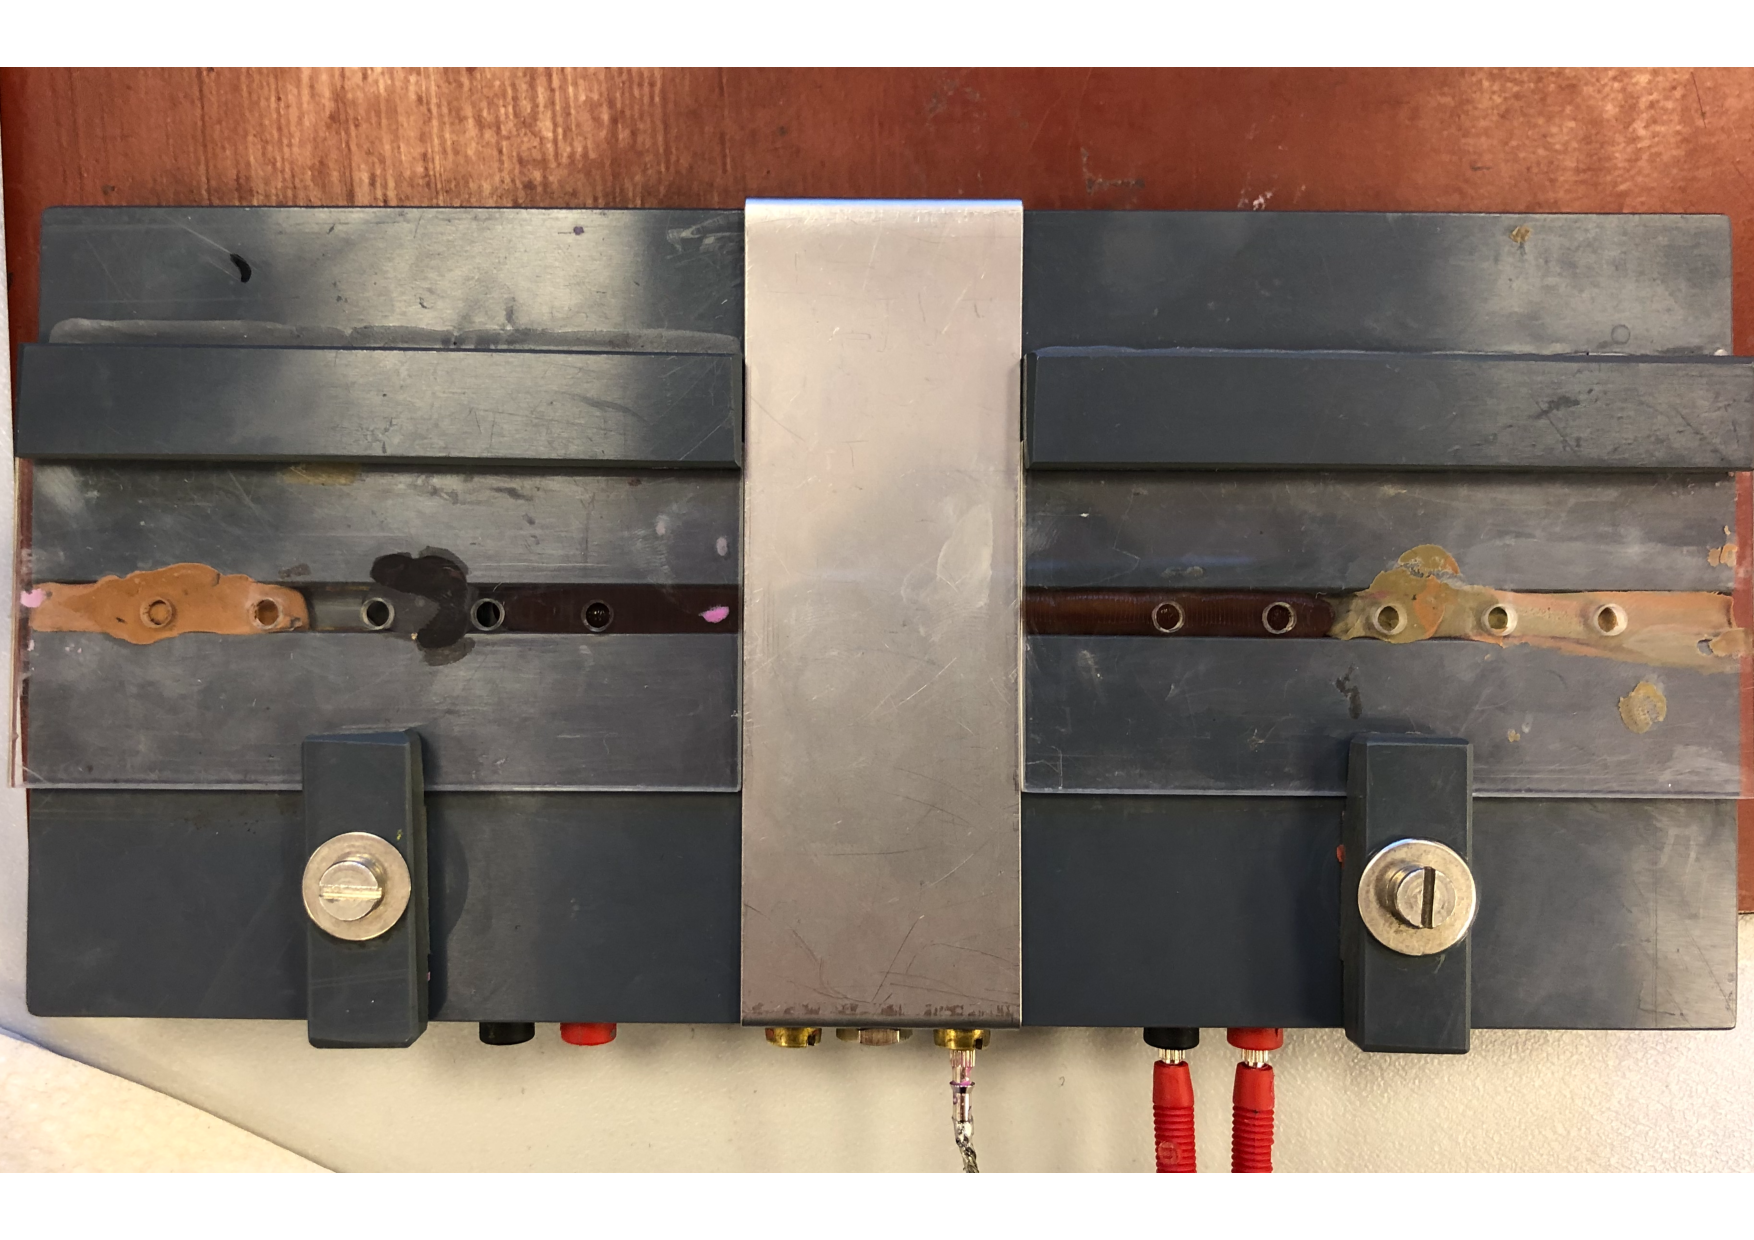
\includegraphics[width=0.8\textwidth]{IMG_6360}}
\caption{Das Bild zeigt, wie der Regenwurm in der Wurmplatte mit Knete und den Plexiglasplatten fixiert wurde. Außerdem sieht man die Verkabelung der Elektroden am posterioren Ende des Wurmes. }
\label{foto}
\end{figure}
\begin{figure}[H]
\makebox[\textwidth][c]{\includegraphics[width=1.3\textwidth]{schema}}
\caption{Die Abbildung zeigt einen schematischen Versuchsaufbau für den 1. - 3. Versuch. Gezeigt sind die verwendeten Komponenten und entlang der Pfeile ist der Informationsfluss zu erkennen. In blauer Schrift sind die Funktionen gekennzeichnet. }
\label{schema}
\end{figure}


\subsection{Versuchsdurchführung}

\subsubsection{Beobachtung der Lokomotion}
In diesem ersten Teil des Versuches wurde der Regenwurm auf ein feuchtes Filterpapier gelegt und seine natürlichen Bewegungen beobachtet.\\
Anschließend wurde mit einem stumpfen Gegenstand mal das anteriore und mal das posteriere Ende gereizt um die jeweiligen Ausweich- bzw. Meidereaktionen beobachten zu können. 

\subsubsection{Identifikation der Riesenfaser bei mechanischer Reizung}
Das Versuchstier wurde in der Wurmplatte fixiert (s. Versuchsaufbau) und ebenfalls mit einem stumpfen Gegenstand je fünf mal am anterioren und posterioren Ende gereizt. Dieses Mal wurde dabei eine differentielle Ableitung mit den Elektroden in der Wurmplatte durchgeführt und aufgezeichnet. Der Moment des Reizes wurde mit einem Keyboardmarker in Spike2 festgehalten. Zwischen zwei Reizen wurden dem Regenwurm je mindestens 30 Sekunden Ruhe gewährt.

\subsubsection{Bestimmung der Reizschwelle und der Fortleitungsgeschwindigkeit von MRF und LRF durch elektrische Reizung}\label{durchführung3}
In diesem Versuchsteil wurde zusätzlich der Reizgenerator an die Wurmplatte angeschlossen, sodass eine elektrische Reizung des Wurm möglich war (siehe Abbildung \ref{schema}). Die Reizelektroden wurden dafür am anterioren Ende des Wurmes angeschlossen. \\
Mit einer Reizdauer von $0.15$ms wurde der Wurm beginnend mit $0.5$V elektrisch gereizt.  Die Spannungsstärke wurde dann in Schritten von $0.5$V inkrementiert, bis zu einer maximalen Reizstärke von $10V$. \\
Die Reizstärke und der Zeitpunkt der Reizung wurden mittels Keyboardmarkern in Spike2 entsprechend markiert. \\
Der Zeitpunkt an dem zuerst ein Aktionspotential beobachtet werden konnte wurde protokolliert. \\


\textbf{Anmerkung}\\
Den folgenden Versuchsteil konnten wir am Versuchstag aufgrund von Zeitmangel durch Komplikationen bei den Messungen leider nicht mehr durchführen. Deshalb werden diese Experimente nur theoretisch beschrieben, fallen im Ergebnisteil weg und werden in der Diskussion auch theoretisch erörtert. 



\subsubsection{Bestimmung der Refraktärphasen bei elektrischer Reizung}
Hier hätte der gleiche Versuchsaufbau wie in Abschnitt \ref{durchführung3} verwendet werden sollen. Der Wurm hätte mittels des Reizgenerators elektrisch gereizt werden sollen und gleichzeitig wäre eine differentielle Ableitung über die Elektroden erfolgt. \\
Diesmal wäre aber die Reizstärke konstant geblieben, während man dagegen aber eine Reizung mit der Einstellung \glqq Twin Pulse\grqq{} durchgeführt hätte, d.h. zwei kurz aufeinanderfolgende Reize. \\
Beginnend mit einem Delay (Abstand zwischen den beiden Reizen) von $20$ms hätte man den Regenwurm elektrisch gereizt. Diesen zeitlichen Abstand hätte man schrittweise dekrementiert, bis man nur noch ein einziges Aktionspotential beobachtet hätte. \\
Anschließend hätte man bei gleichbleibendem Delay die Reizstärke wieder schrittweise inkrementiert, bis man wieder ein zweites Aktionspotential beobachtet hätte. Zuletzt hätte man erneut den Delay bei gleichbleibender Reizstärke dekrementiert, bis wieder nur ein Aktionspotential zu beobachten gewesen wäre. 


\section{Ergebnisse}
Durch verschiedene Störfaktoren enthalten unsere Messungen leider viele Artefakte und sind zum Teil unvollständig.  \\
Die Dokumentation des Reizmoments für die Bestimmung der Latenzzeit konnte nicht mit ausreichender Genauigkeit erfolgen, sodass diese Daten im folgenden Ergebnis-Teil fehlen. \\

\subsection{Beobachtung der Lokomotion}
Wir konnten beobachten, dass sich der Wurm zur Fortbewegung zuerst nach vorne ausstreckte und anschließend den hinteren Teil des Körpers nach- und sich so zusammenzog. Hierbei entfernten sich die Segmente bei der Streckung voneinander, um beim Zusammenziehen wieder ineinander zu gleiten.\\
Leider zeigte das Versuchstier nur sehr schwache Meidereaktionen bei Reizung des posterioren oder anterioren Körperendes. Trotzdem konnte man schwach erkennen, dass der Regenwurm bei anteriorer Reizung den Körper zusammenzog und so das Körperende vom Reiz wegbewegte. Bei posteriorer Reizung ließ sich keine eindeutige Vermutung auf Meidereaktion erkennen. 

\subsection{Identifikation der Riesenfaser bei mechanischer Reizung}
Wir wählten eine hundertfache Verstärkung der gemessenen Spannungen.\\
Aufgrund der vielen Artefakte und trotz mehrerer Messungen an drei verschiedenen Versuchstieren, konnten wir in den Messungen lediglich jeweils drei Aktionspotentiale eines Versuchstieres identifizieren und somit auswerten. 

\begin{figure}[H]
\makebox[\textwidth][c]{\includegraphics[width=1.3\textwidth]{aufgabe2/a6_1.png}}
\caption{Ableitung eines extrazellulär abgeleiteten Aktionspotentials nach anteriorer Reizung: In der Abbildung zeigt die grüne Kurve den Verlauf einer extrazellulären, differentiellen Ableitung.  Die Amplitude des identifizierten Aktionspotentials beträgt $0,035-(-0,007)=0,042 mV$ und die Dauer $1,521/2 \approx 0,761 ms$ }
\label{ant}
\end{figure}

\begin{figure}[H]
\makebox[\textwidth][c]{\includegraphics[width=1.3\textwidth]{aufgabe2/p4_2.png}}
\caption{Ableitung eines extrazellulär abgeleiteten Aktionspotentials nach posteriorer Reizung: In der Abbildung zeigt die grüne Kurve den Verlauf einer extrazellulären, differentiellen Ableitung.  Die Amplitude des identifizierten Aktionspotentials beträgt $0,0413-(-0,0036)=0,045 mV$ und die Dauer $2,432/2 \approx 1,216 ms$ }
\label{post}
\end{figure}

In Abbildung \ref{ant} ist beispielhaft die Ableitung eines Aktionspotentials nach anteriorer Reizung zu sehen. Es ist klar zu erkennen, dass die Kurve erst steigt und dann fällt. Handelt es sich um eine posteriore Reizung (siehe Abbildung \ref{post}) so fällt die Kurve zuerst und steigt danach.

\begin{table}[H]
\caption{In der untenstehenden Tabelle sind Amplitude (in mV) und Dauer (in ms) der identifizierten Aktionspotentiale nach anteriorer bzw. posteriorer Reizung dargestellt, sowie der jeweils berechnete Durchschnitt und die Standardabweichung.}
\begin{center}
\begin{tabular}{l||c|c}
Art & Amplitude in mV & Dauer in ms \\
\hline\hline
Anteriorer Reiz & 0,031 & 0,817\\
Anteriorer Reiz & 0,036 & 0,659\\
Anteriorer Reiz & 0,042 & 0,761\\
\hline
Durchschnitt & 0,0363& 0,7457\\
Standardabweichung & 0,00449 &0,0654 \\
\hline\hline
Posteriorer Reiz & 0,032 & 1,206\\
Posteriorer Reiz & 0,026& 1,202\\
Posteriorer Reiz & 0,045 & 1,216\\
\hline
Durchschnitt & 0,0343 & 1,208\\
Standardabweichung & 0,00793& 0,00589
\end{tabular}
\end{center}
\label{werte}
\end{table}

In Tabelle \ref{werte} sind die gemessenen Werte der jeweils 3 Aktionspotentiale dargestellt, sowie die Berechnungen der Dauer und der Standardabweichung. Für die Berechnung der Dauer haben wir, wie in Abbildung \ref{ant} und Abbildung \ref{post} zu sehen, die Marker auf den Anfang und das Ende der S-Kurve gesetzt und den resultierenden Wert durch zwei geteilt, um ein genaueres Ergebnis zu erhalten.\\
Allgemein lässt sich erkennen, dass die Größe der Amplituden bei anterioren und posterioren Reizen nahezu identisch ist, der Durchschnitt weist lediglich einen Unterschied von $0,002 mV$ auf. Allerdings ist die Dauer bei den posterioren Reizen im Durchschnitt um $0,4623 ms$ länger.


\subsection{Bestimmung der Reizschwelle und der Fortleitungsgeschwindigkeit von MRF und LRF durch elektrische Reizung}
Die ersten Aktionspotentiale konnten bei einer Reizstärke von 3,5 V erkannt werden. Leider war es aufgrund der vielen Artefakte nicht möglich zu erkennen, bei welcher Reizung zwei Aktionspotentiale auftreten. Die Ergebnisse sind demnach unvollständig. 

\begin{figure}[H]
\makebox[\textwidth][c]{\includegraphics[width=1.3\textwidth]{aufgabe3/g2.png}}
\caption{Ableitung eines extrazellulär abgeleiteten Aktionspotentials nach elektrischer Reizung: In der Abbildung zeigt die grüne Kurve den Verlauf einer extrazellulären, differentiellen Ableitung.  Die Amplitude des identifizierten Aktionspotentials beträgt $0,158 mV$ und die Dauer $0,1/2 \approx 0,05 s$. Anmerkung: In der Abbildung sind die y-Achsen gespiegelt.}
\label{g2}
\end{figure}

Wie in Abbildung \ref{g2} zu erkennen ist, enthält auch diese Ableitung viele Störungen und Schwankungen, was die Identifikation der Aktionspotentiale erschwerte. Die in Tabelle \ref{werte2} dargestellten und ausgewerteten Werte stammen von dem in Abbildung \ref{g2} abgebildeten sowie einem weiteren Aktionspotential, das identifiziert werden konnte.

\begin{table}[H]
\caption{In der untenstehenden Tabelle sind die Amplitude (in mV), Dauer und Latenzzeit (jeweils in s) der zwei identifizierten Aktionspotentiale nach elektrischer Reizung mit einer Reizstärke von $3,5V$ dargestellt, sowie der jeweils berechnete Durchschnitt und die Standardabweichung.}
\begin{center}
\begin{tabular}{l||c|c|c}
Art & Amplitude in mV & Dauer in s & Latenzzeit in s\\
\hline\hline
 Reiz 1& 0,168 & 0,0298 & 0,134\\
Reiz 2& 0,158 & 0,05 & 0,114\\
\hline
Durchschnitt & 0,163 & 0,0399 & 0,124\\
Standardabweichung & 0,0035 &0,00714 & 0,0071
\end{tabular}
\end{center}
\label{werte2}
\end{table}

%\begin{figure}[H]
%\makebox[\textwidth][c]{\includegraphics[width=1.3\textwidth]{aufgabe3/g2.png}}
%\caption{Ableitung eines extrazellulär abgeleitetem Aktionspotential nach elektrischer Reizung: In der Abbildung ist in Grün der Verlauf einer extrazellulären differentiellen Ableitung zu sehen.  Die Amplitude des identifizierten Aktionspotential beträgt $0,168 mV$ und die Dauer $0,0595 s$}
%\label{g2}
%\end{figure}

\subsection{Bestimmung der Refraktärphasen bei elektrischer Reizung}
Diesen Versuch konnten wir aufgrund von Zeitmangel nicht durchführen. Theoretisch erwartete Ergebnisse werden in der Diskussion erläutert.

\section{Diskussion}

\textbf{1. Versuch} \\
Im ersten Teil des Experimentes wurden die Kriechbewegungen und Meidereaktionen des Regenwurmes beobachtet. 
Das Fehlen eindeutiger Meidereaktionen könnte daran liegen, dass der Wurm an diesem Tag schon von anderen Gruppen in mehreren Versuchen verwendet wurde. \\
Erwartete Meidereaktionen waren das Zusammenziehen des entsprechenden Körperendes (siehe Abschnitt \ref{anatomie}). \\

\textbf{2. Versuch}\\
Die Aufzeichnungen der differentiellen Ableitung während anteriorer und posteriorer Reizung des Wurmes zeigen die Aktivierung der MRF bzw. LRF dabei. \\
Da wir eine differentielle Ableitung durchgeführt haben, sehen wir immer die Differenz der Spannungen zwischen den Elektroden. Diese Differenz lässt Rückschlüsse auf die Richtung des Aktionspotentials und damit auf die aktivierte Riesenfaser (MRF oder LRF) zu. \\
Wie in Abschnitt \ref{differentiell} erläutert, lässt sich die Gesamtspannung bei der differentiellen Ableitung aus $U_{ges} \approx U_1 - U_2$ berechnen. \\

In Abbildung \ref{ant} ist zu sehen, dass die MRF aktiv ist wenn der Wurm am anterioren Ende gereizt wurde. Die Kurve schlägt erst nach oben aus, dann nach unten. D.h. die Spannung wird erst positiver wenn das Aktionspotential an der zweiten Elektrode vorbeiläuft, geht zurück auf $0V$, wenn das Aktionspotential in der Mitte der Elektroden angekommen ist und zeigt dann eine negative Spannung, wenn das Aktionspotential an der ersten Elektrode angekommen ist. \\
Entsprechend zeigt Abbildung \ref{post} eine Umkehrung dieser Ausschläge. Da die Reizung am posterioren Ende die LRF aktiviert, zeigt sich zuerst eine negative Spannung und danach eine positive Spannung. D.h. das Aktionspotential läuft hier genau in die entgegengesetzte Richtung als bei der Reizung am anterioren Ende. \\
Die Unterschiede in der Dauer der Aktionspotentiale (anterior durchschnittlich $0.7457ms$, posterior durchschnittlich $1,208ms$) könnten darauf hindeuten, dass es sich bei den lateralen Riesenfasern um zwei \glqq synchronisierte\grqq{} Neurone handelt. Bei Aktivierung der LRF war die Dauer größer als bei der MRF. Da wir eine extrazelluläre Messung durchgeführt haben, kann es sein, dass es durch die Summation der Aktionspotentiale aus den beiden LRF zur Beobachtung längerer Aktionspotentiale kam. \\
Die Amplituden der Aktionspotentiale zeigten keine großen Differenzen (Unterschied Durchschnitt $0,002mV$) zwischen anteriorer und posteriorer Reizung. Bei der anterioren Reizung wird zwar nur die Aktivität einer einzigen Riesenfaser gemessen (MRF), diese hat aber einen größeren Durchmesser als die beiden LRF, dessen Aktivität bei der posterioren Reizung aufgezeichnet wird. Bei den lateralen Riesenfasern kommt es zur Summation (extrazelluläre Messung), sodass wir ähnliche Amplituden beobachtet haben. \\
Bezüglich der Latenzzeit würde man erwarten, dass diese bei der anterioren Reizung, d.h. bei Aktivierung der MRF geringer sein würde, da die MRF einen größeren Durchmesser hat als die LRF, sodass der Längswiderstand kleiner ist. \\

%$\rightarrow$ 520 Wörter, maximal 800 ? 

\textbf{3. Versuch}\\
Die gemessenen Werte in Tabelle \ref{werte2} zeigen die Amplitude (mV), Dauer und Latenzzeit (jeweils in Sekunden) von Aktionspotentialen des Wurms bei elektrischen Reizen mit 3,5V Stärke.\\
Da unsere Messungen viele Artefakte enthielten, fiel es uns schwer Aktionspotentiale vernünftig erkennen und auswerten zu können. Die Anzahl und schwere der Artefakte liegt zum Einen an der Art der Ableitung, da extrazelluläre Ableitungen anfälliger für Störungen sind als intrazelluläre. Zusätzlich sondern Regenwürmer in bedrohlichen Situationen Schleim ab, der wenn er die Elektroden benetzt, eine klare Ableitung fast unmöglich macht. Mehrere Versuche, die Störungen zu minimieren waren erfolglos.\\
Bei den Messwerten (siehe Tabelle \ref{werte2}) fällt sofort ins Auge, dass die Zahlen stark von den im zweiten Versuch gemessenen Werten (siehe Tabelle \ref{werte}) abweichen. Während die Amplitude ca. 4,5 mal so hoch ist wie die durchschnittliche Amplitude in Tabelle \ref{werte}, ist die Dauer sogar zwischen 24 und 67 mal so hoch wie die im vorherigen Versuchsteil gemessenen Werte.\\
Dies könnte daran liegen, dass die von uns als Aktionspotentiale identifizierten Kurven lediglich Störungen waren.\\

\textbf{4. Versuch}\\
Dieser Versuch sollte durch zwei kurz aufeinanderfolgende Reize mit verändertem zeitlichen Abstand zur Ermittlung der Refraktärphase dienen. \\
Verringert man den Delay (die Verzögerung), sollte man ab einem Schwellenwert nicht mehr zwei, sondern nur noch ein Aktionspotential beobachten können. Dies ist auf die Inaktivierung der Natrium-Kanäle in der Refraktärphase zurückzuführen (siehe Abschnitt \ref{refraktär}). \\
Bei anschließender Erhöhung der Reizstärke mit gleichbleibender Verzögerung, bis man wieder ein zweites Aktionspotential beobachten kann, erhält man einen neuen Schwellenwert, bei dem es sich um den Beginn der relativen Refraktärphase $t_2$ handelt. Während dieser Phase ist eine Öffnung der Natrium-Kanäle möglich, benötigt aber ein höheres Schwellenpotential. Hier ist auch eine Verringerung der Amplitude der Aktionspotentiale zu erwarten. \\
Wenn man schließlich wieder den Delay verringert, bis man kein zweites Aktionspotential mehr beobachtet, erhält man den Beginn der absoluten Refraktärphase $t_1$. Dies ist die Phase, in der überhaupt kein Aktionspotential ausgelöst werden kann, da die Natrium-Kanäle noch inaktiv sind. \\
D.h. die die absolute Refraktärphase dauert $t_1$ an und die relative Refraktärphase $t_2-t_1$. \\
Die maximale Aktionspotential-Frequenz ergibt sich aus der absoluten Refraktärzeit. Ausgehend von einer realistischen absoluten Refraktärzeit von $2ms$ erhält man eine maximal mögliche AP-Frequenz von $500Hz$. 





\begin{thebibliography}{999}
\bibitem {lehninger} Nelson, David; Cox, Michael: Lehninger Biochemie. Springer Verlag, 2011.
\bibitem {zellbiologie} Karp, Gerald: Molekulare Zellbiologie. Springer Verlag, 2005.
\bibitem {haustiere} von Engelhardt, Wolfgang: Physiologie der Haustiere. Georg Thieme Verlag, 2010. 
\bibitem {physiologie} Schmidt, Robert; Lang, Florian; Heckmann, Manfred: Physiologie des Menschen, mit Pathopyhsiologie. Springer Medizin Verlag, 2010. 
\bibitem{koerperbau} \url{http://www.regenwuermer.info/regenwurm/regenwurm-koerperbau.php} \\Zugriff 18.01.2019 14:20 Uhr
\bibitem{skript} Skript: Erregungsleitung im Bauchmark des Regenwurms

\bibitem [Abbildung 1]{Abb1} \url{https://www.repetico.de/card-16616620}, \\Zugriff 17.01.2019 13:20 Uhr
\bibitem [Abbildung 2]{Abb2} Karp, Gerald: Molekulare Zellbiologie. Springer Verlag, 2005.
\bibitem [Abbildung 3]{bauchmark} \url{https://hypersoil.uni-muenster.de/1/02/26.htm}, \\Zugriff 18.01.2019 12:13 Uhr
\end{thebibliography}


\end{document}
